\documentclass{article}

\usepackage{amsfonts}
\usepackage{amsmath}
% \usepackage{svg} %For including svgs
% \svgpath{{../assets/}}
\usepackage{graphicx}
\graphicspath{ {../assets/} }
\usepackage[margin=1in]{geometry} %Change margins
\usepackage{hyperref} %For hyperlinks in table of contents and other
\usepackage{float} %For using H in figure
\usepackage{subcaption} %For subfigures
\usepackage{booktabs} %For tables
\usepackage{multirow} %For tables

\usepackage[charsperline=120]{jlcode} %For Julia Code Listing https://github.com/wg030/jlcode

\addtolength{\jot}{1em} %https://tex.stackexchange.com/questions/14679/amsmath-align-environment-row-spacing

\title{Optimization Assignment 2\\Computation Effort Comparison between Zero-Order, First-Order, and Second-Order Optimization Algorithms}
\date{Winter 2021}
\author{Kim Paolo Laberinto (7771083)}

\begin{document}
    \maketitle
    \newpage

    \tableofcontents
    \newpage


    \section{Methodology}

    In this report several optimization algorithms were run on the 5D Rosenbrock function, with various initial guess vectors.
    The initial guess vectors used in this report can be in Table \ref{tab:initial_vectors}. 

    \begin{table}[H]
        \centering
        \begin{tabular}{@{}ll@{}}
        \toprule
                                  & \textbf{Vector}                     \\ \midrule
        \textbf{Initial Vector 1} & [ 0.00,  0.00,  0.00,  0.00,  0.00] \\
        \textbf{Initial Vector 2} & [ 0.36,  1.18, -1.01, -1.73, -0.90] \\
        \textbf{Initial Vector 3} & [ 1.07,  1.42,  0.32,  1.83,  0.61] \\
        \textbf{Initial Vector 4} & [ 0.26, -1.20,  0.60,  0.59, -1.77] \\
        \textbf{Initial Vector 5} & [-0.16, -0.81, -1.96, -1.55,  1.37] \\ \bottomrule
        \end{tabular}
        \caption{Table of Initial Vectors used for analysing performance}
        \label{tab:initial_vectors}
    \end{table}

    The equation for the 5D Rosenbrock function is below. 
    For some algorithms, the gradient and hessian of the 5D Rosenbrock function were also required.
    Autodifferentiation techniques using ForwardDiff.jl were used to get the gradient and hessian.

    \begin{equation}
        f(x) = \sum_{i = 1}^{5 - 1} 100(x_{i+1} - x_i^2)^2 + (1-x_i)^2
    \end{equation}

    Each of the algorithms were measured using different metrics such as:
    \begin{itemize}
        \item Number of Function Evaluations
        \item Number of Gradient Function Evaluations
        \item Number of Hessian Function Evaluations
        \item Number of Linear System Solves (e.g. inversions and similar)
        \item Run-time
        \item Percentage Time Spent in Garbage Collection
    \end{itemize}

    The remainder of this report showcases the various Loss vs Iteration plots for each of the algorithms with a short commentary.
    The final concluding sections of this report show the metrics measured on each algorithm.

    \subsection{Limitations}

    Note that this report is solely for educational purposes only in possible methods of analysis, 
    and not meant to be used to rigorously compare the various algorithms. 
    
    For example, timing measurements in Table \ref{tab:concludingtimings} also include the time for recording trial data/metrics such as loss vs iterations and saving hessian matrices for further analysis. 
    These things may have a significant impact on memory allocation and run-time. In this report, these effects are not excluded.

    Performance is also highly dependent on the implementation of the algorithm itself.
    The algorithm implementations written by the author used in this report are not optimized for time or memory usage.

    \subsection{Further Areas to Explore}

    There are more opportunities in analyzing these algorithms. Potential areas of analysis include:

    \begin{itemize}
        \item Optimizing for memory use and allocation to see its impact on performace
        \item Profiling the code to examine which lines run the longest
        \item Controling and comparing the hyperparameters across algorithms (gradient tolerences, max iterations, etc.)
        \item Increasing the number of parameters and solving much bigger optimization problems
    \end{itemize}

    \section{Algorithm Performances - Loss vs Iterations}

    In this section, the Loss vs Iterations plots for each algorithm can be seen.
    Short commentaries can be found in the subsections below discussing the results seen in the plots.
    \subsection{Steepest Descent}

    As seen in Fig. \ref{fig:GradientDescentLossPlot.png}, 
    this naive technique took a significant amount of iterations to reach the stopping condition $\| \nabla f \| = 10^{-4}$.
    The author hypothesizes that this may be due to a "zig-zag" descent pattern in the steep valleys of the objective function.
    Each iteration in the gradient descent only lowers the loss by a small amount (relative to the other more efficient algorithms below).

    \begin{figure}[H]
        \centering
        \includegraphics[width=0.5\linewidth]{GradientDescentLossPlot.png}
        \caption{Gradient Descent Loss vs Iterations Plot}
        \label{fig:GradientDescentLossPlot.png}
    \end{figure}

    \subsection{Powell's Conjugate Direction}

    Powell's Conjugate Direction on Initial Vector 2 had to abort due to facing a Case 4: Non-Unimodal error in the Swann's Bracketing Method algorithm as discussed in the notes/pseudocode. The implementation aborted, leaving the run for Initial Vector 2 with only a very short run.

    The other runs with the other initial vectors stopped without any errors upon reaching the stopping condition specified in the code.

    \begin{figure}[H]
        \centering
        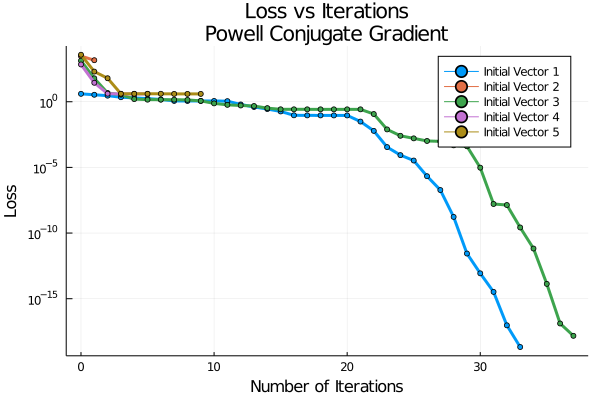
\includegraphics[width=0.5\linewidth]{PowellConjugateGradient_LossPlot.png}
        \caption{Powells Conjugate Directions Loss vs Iterations}
        \label{fig:PowellConjugateGradient_LossPlot.png}
    \end{figure}

    \subsection{Conjugate Gradient Techniques}

    As seen in Fig. \ref{fig:ConjugateGradientFletcherReeves_LossPlot.png}, 
    the Fletcher-Reeves Conjugate Gradient algorithm reached a loss in the order of $10^{-10}$ to $10^{-20}$ to the stopping condition $\| \nabla f \| = 10^{-4}$ in only 40 - 80 iterations. Whereas the Hestenes-Stiefel and Polak-Ribi\`ere variations of the Conjugate Gradient method took much longer to reach the same stopping condition.

    \subsubsection{Fletcher-Reeves}
    \begin{figure}[H]
        \centering
        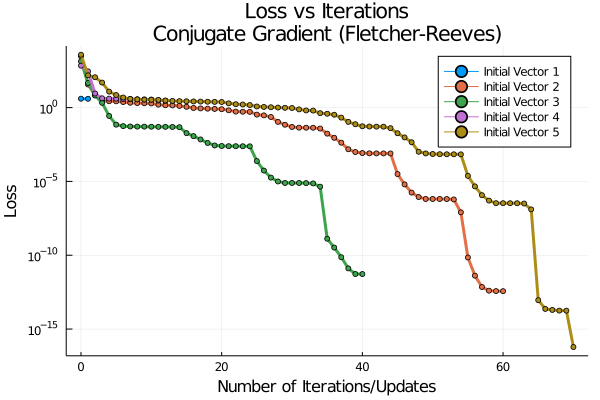
\includegraphics[width=0.5\linewidth]{./ConjugateGradientFletcherReeves_LossPlot.png}
        \caption{Fletcher-Reeves Conjugate Gradient - Loss vs Iterations}
        \label{fig:ConjugateGradientFletcherReeves_LossPlot.png}
    \end{figure}
    
    \subsubsection{Hestenes-Stiefel}
    \begin{figure}[H]
        \centering
        \includegraphics[width=0.5\linewidth]{./ConjugateGradientHestenesStiefel_LossPlot.png}
        \caption{Hestenes-Stiefel Conjugate Gradient - Loss vs Iterations}
        \label{fig:ConjugateGradientHestenesStiefel_LossPlot.png}
    \end{figure}
    
    \subsubsection{Polak-Ribi\`ere}
    \begin{figure}[H]
        \centering
        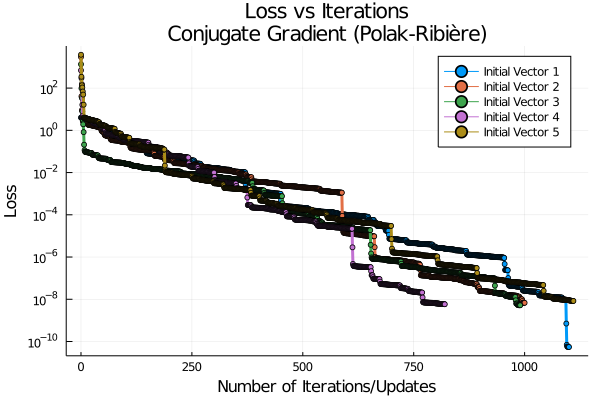
\includegraphics[width=0.5\linewidth]{./ConjugateGradientPolakRibiere_LossPlot.png}
        \caption{Polak-Ribi\`ere Conjugate Gradient - Loss vs Iterations}
        \label{fig:ConjugateGradientPolakRibiere_LossPlot.png}
    \end{figure}

    \subsection{Hooke-Jeeves Direct Search}

    \begin{figure}[H]
        \centering
        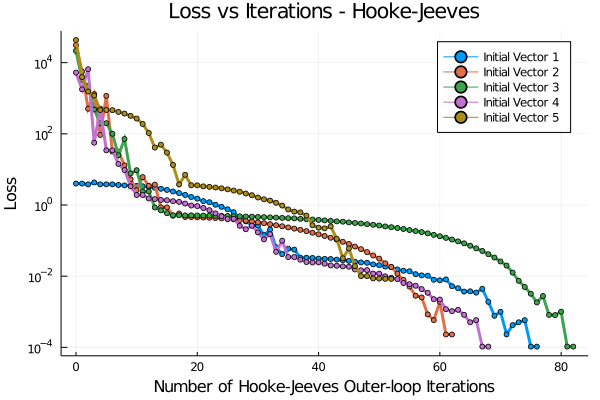
\includegraphics[width=0.5\linewidth]{./HookeJeevesLossPlot.png}
        \caption{Hooke-Jeeves - Loss vs Iterations}
        \label{fig:HookeJeevesLossPlot.png}
    \end{figure}

    \subsection{Nelder-Mead Simplex Search}

    The stopping condition for this implementation of Nelder-Mead was to reach 500 iterations. As seen in Fig. \ref{fig:NelderMead_LossPlot.png}, after 500 iterations, a loss of $10^1$ to $10^{-3}$ was achieved. This is relatively inefficient algorithm in terms of amount of iterations and lowest loss achieved compared to the other algorithms in this report.

    \begin{figure}[H]
        \centering
        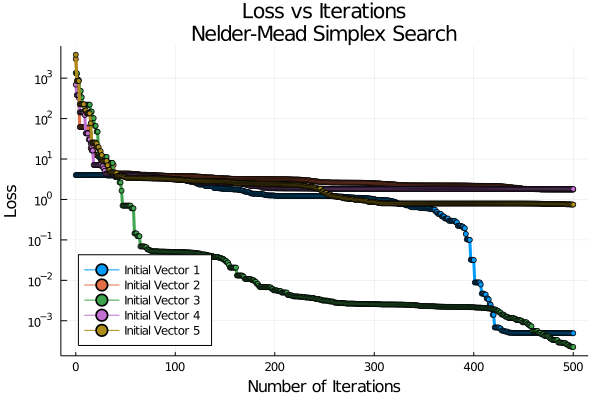
\includegraphics[width=0.5\linewidth]{./NelderMead_LossPlot.png}
        \caption{Nelder-Mead - Loss vs Iterations}
        \label{fig:NelderMead_LossPlot.png}
    \end{figure}

    \subsection{Original Newton's Method}

    The update equation for Newton's Method is seen in the equation below.

    \begin{equation}
        x_{k+1} = x_k - H_k^{-1} g_k
    \end{equation}

    The stopping condition for this implementation of the Original Newton's Method is reaching a  $\| \nabla f \| = 10^{-3}$.

    As seen in Fig. \ref{fig:OriginalNewtonsMethod_LossPlot.png}, all initial starting vectors reached a loss of $10^{-10}$ to $10^{-25}$ in 25 iterations or less. This shows an efficient algorithm in terms of iterations.

    \begin{figure}[H]
        \centering
        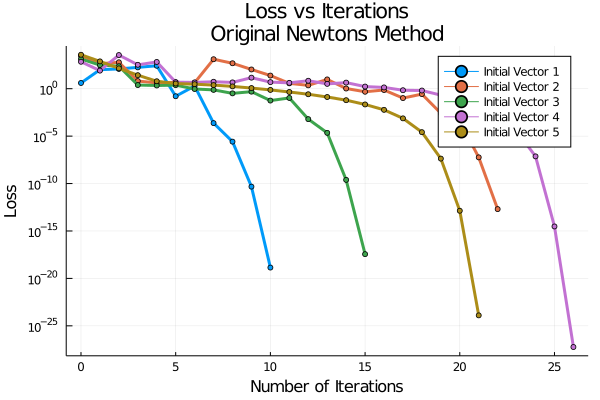
\includegraphics[width=0.5\linewidth]{./OriginalNewtonsMethod_LossPlot.png}
        \caption{Original Newtons Method - Loss vs Iterations}
        \label{fig:OriginalNewtonsMethod_LossPlot.png}
    \end{figure}

    \begin{figure}[H]
        \centering
        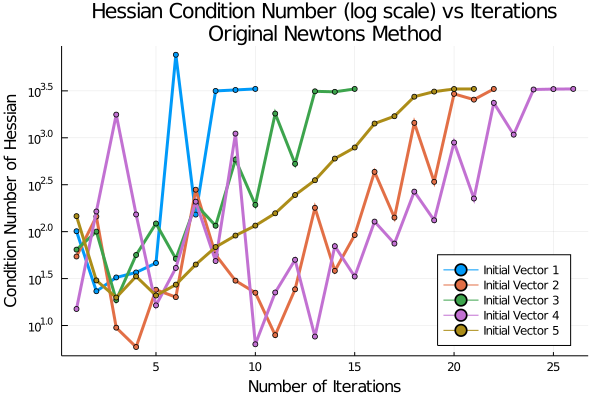
\includegraphics[width=0.5\linewidth]{./OriginalNewtonsMethod_ConditionNumberHessianPlot.png}
        \caption{Original Newtons Method - Condition Number of Hessian vs Iteration}
        \label{fig:OriginalNewtonsMethod_ConditionNumberHessianPlot.png}
    \end{figure}

    \subsection{Modified Newton's Method with Levenberg-Marquardt Modification}

    The algorithm in this section uses the following update equation.

    \begin{equation}
        x_{k+1} = x_k - \alpha (H_k + \mu I)^{-1} g_k
    \end{equation}

    Where $\alpha_k$ was determined from a line search. i.e.

    \begin{equation}
        \alpha_k = \text{argmin}_{\alpha} f(x_k + \alpha d_k)
    \end{equation}

    In this section different mu values were analyzed.
    \begin{itemize}
        \item $\mu = 0.0$
        \item $\mu = 1.0$
        \item $\mu = 10.0$
    \end{itemize}

    \subsubsection{Loss vs Iterations}
    
    As one can see in this section, $\mu = 0.0$ performed the best out of the other $\mu$ parameters.
    The author hypothesizes that this is due to the fact that the 5-D Rosenbrock function contains many valleys where gradient descent can zig-zag and get stuck on.

    The $\mu = 10.0$ case looks similar to the Gradient Descent method above in Fig \ref{fig:GradientDescentLossPlot.png}, with a slow descent and taking many iterations. 
    The author hypothesizes that this is due to the common "zig-zag" effect with Gradient Descent methods.

    \begin{figure}[H]
        \centering
        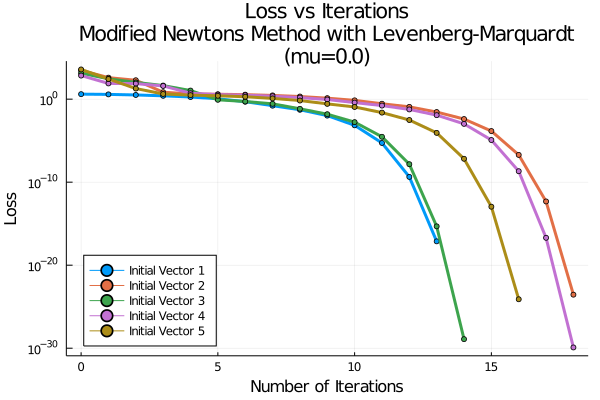
\includegraphics[width=0.5\linewidth]{./ModifiedNewtons/ModifiedNewtonsWithLM_LossPlot_1.png}
        \caption{Modified Newton's method - Loss vs Iterations (mu = 0.0)}
        \label{fig:ModifiedNewtonsWithLM_LossPlot_1.png}
    \end{figure}
    
    \begin{figure}[H]
        \centering
        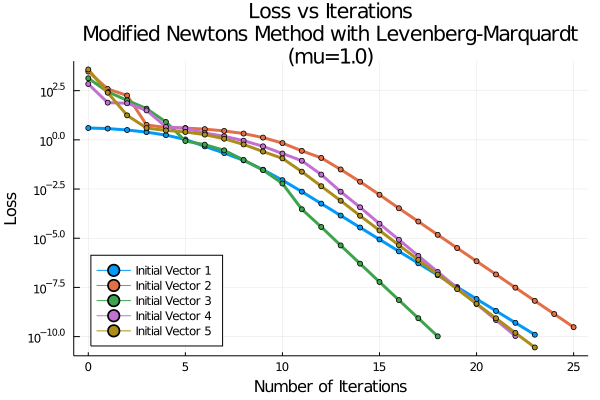
\includegraphics[width=0.5\linewidth]{./ModifiedNewtons/ModifiedNewtonsWithLM_LossPlot_2.png}
        \caption{Modified Newton's method - Loss vs Iterations (mu = 1.0)}
        \label{fig:ModifiedNewtonsWithLM_LossPlot_2.png}
    \end{figure}
    
    \begin{figure}[H]
        \centering
        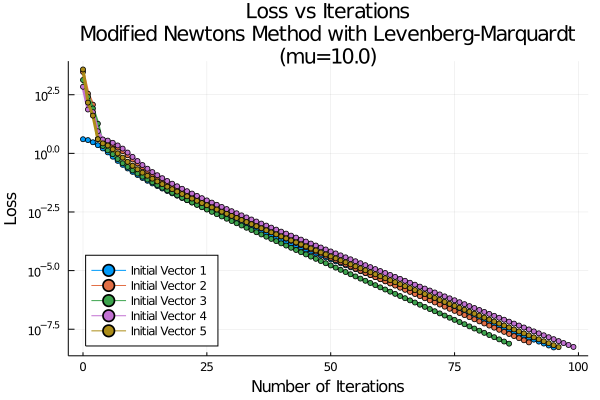
\includegraphics[width=0.5\linewidth]{./ModifiedNewtons/ModifiedNewtonsWithLM_LossPlot_3.png}
        \caption{Modified Newton's method - Loss vs Iterations (mu = 10.0)}
        \label{fig:ModifiedNewtonsWithLM_LossPlot_3.png}
    \end{figure}

    \subsubsection{Condition Number of LM-Matrix}

    In this section, the LM-Matrix denotes the $(H_k + \mu I)$ i.e the sum of the Hessian Matrix with the diagonal $\mu$-parameter matrix.

    \begin{figure}[H]
        \centering
        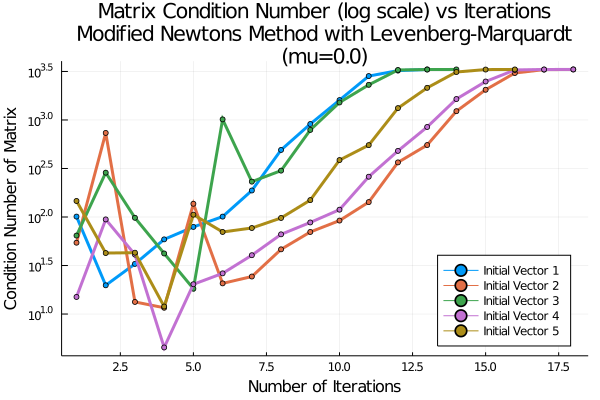
\includegraphics[width=0.5\linewidth]{./ModifiedNewtons/ModifiedNewtonsWithLM_ConditionNumberHessianPlot_1.png}
        \caption{Condition Number of LM-Matrix vs Iterations (mu = 0.0)}
        \label{fig:ModifiedNewtonsWithLM_ConditionNumberHessianPlot_1.png}
    \end{figure}
    
    \begin{figure}[H]
        \centering
        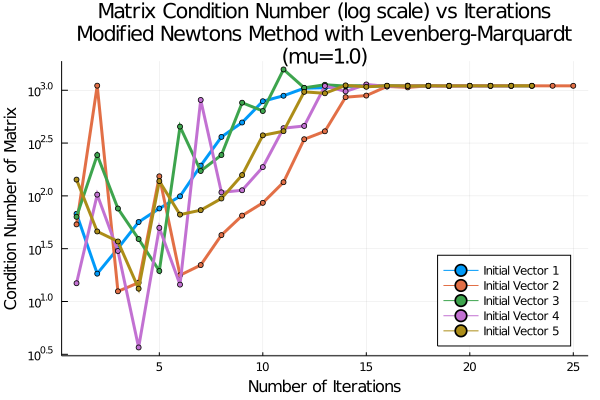
\includegraphics[width=0.5\linewidth]{./ModifiedNewtons/ModifiedNewtonsWithLM_ConditionNumberHessianPlot_2.png}
        \caption{Condition Number of LM-Matrix vs Iterations (mu = 1.0)}
        \label{fig:ModifiedNewtonsWithLM_ConditionNumberHessianPlot_2.png}
    \end{figure}
    
    \begin{figure}[H]
        \centering
        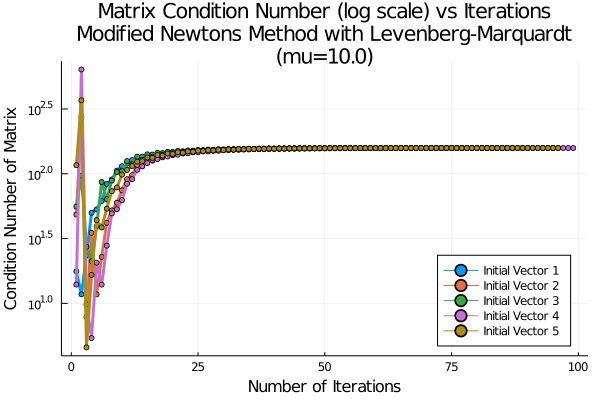
\includegraphics[width=0.5\linewidth]{./ModifiedNewtons/ModifiedNewtonsWithLM_ConditionNumberHessianPlot_3.png}
        \caption{Condition Number of LM-Matrix vs Iterations (mu = 10.0)}
        \label{fig:ModifiedNewtonsWithLM_ConditionNumberHessianPlot_3.png}
    \end{figure}

    
    \section{Metric Comparisons between Algorithms}

    Table \ref{tab:concludingmetrics} contains a summary of all the metric performances of all the algorithms for Initial Vector 1.
    Table \ref{tab:concludingtimings} contains the runtime measured for each algorithm on Initial Vector 1. Multiple samples were taken.
    Only one initital vector was used for this section with Metrics and Timings.

    \begin{table}[H]
    \centering
    \begin{tabular}{@{}llllll@{}}
    \toprule
     &
      \begin{tabular}[c]{@{}l@{}}Count\\ f evals*\end{tabular} &
      \begin{tabular}[c]{@{}l@{}}Count\\ grad\_f evals\end{tabular} &
      \begin{tabular}[c]{@{}l@{}}Count\\ hessian\_f evals\end{tabular} &
      \begin{tabular}[c]{@{}l@{}}Count\\ inverse solves\end{tabular} &
      \begin{tabular}[c]{@{}l@{}}Final\\ Loss\end{tabular} \\ \midrule
    Steepest/Gradient Descent           & 330625 & 11809 & 0  & 0  & 7.50E-9  \\
    Powell's Conjugate Direction        & 5111   & 0     & 0  & 0  & 2.09E-19 \\
    Fletcher-Reeves Conjugate Gradient  & 1      & 2047  & 0  & 0  & 2.08E-17 \\
    Hestenes-Stiefel Conjugate Gradient & 1      & 30991 & 0  & 0  & 8.40E-9  \\
    Polak-Ribi\`ere Conjugate Gradient  & 1      & 34976 & 0  & 0  & 1.38E-9  \\
    Hooke-Jeeves Direct Search          & 1176   & 0     & 0  & 0  & 1.05E-4  \\
    Nelder-Mead Simplex Search          & 3501   & 0     & 0  & 0  & 4.91E-4  \\
    Original Newtons Method             & 1      & 11    & 10 & 10 & 1.39E-19 \\
    Modified Newton with LM (mu = 0.0)  & 1      & 97    & 13 & 13 & 7.44E-18 \\
    Modified Newton with LM (mu = 1.0)  & 1      & 141   & 23 & 23 & 1.25E-10 \\
    Modified Newton with LM (mu = 10.0) & 1      & 462   & 95 & 95 & 5.28E-9  \\ \bottomrule
    \end{tabular}
    \caption{Metric Comparison for all Algorithms for Initial Vector 1. Note that all algorithms has one additional f-evaluation performed to determine the final loss.}    
    \label{tab:concludingmetrics}
    \end{table}

    \begin{table}[H]
    \centering
    \resizebox{\textwidth}{!}{%
    \begin{tabular}{@{}lrrrrrrl@{}}
    \toprule
     &
      \begin{tabular}[c]{@{}l@{}}Min.\\ Time\end{tabular} &
      \begin{tabular}[c]{@{}l@{}}Min.\\ Time\\ \% GC\end{tabular} &
      \begin{tabular}[c]{@{}l@{}}Median\\ Time\end{tabular} &
      \begin{tabular}[c]{@{}l@{}}Median\\ Time\\ \% GC\end{tabular} &
      \begin{tabular}[c]{@{}l@{}}Max.\\ Time\end{tabular} &
      \begin{tabular}[c]{@{}l@{}}Max.\\ Time\\ \% GC\end{tabular} &
      \begin{tabular}[c]{@{}l@{}}Final\\ Loss\end{tabular} \\ \midrule
    Steepest/Gradient Descent           & 4.110 s    & 11.42\% & 4.112 s    & 11.58\% & 4.115 s    & 11.73\% & 7.50E-9  \\
    Powell's Conjugate Direction        & 57.033 ms  & 0.00\%  & 66.822 ms  & 12.67\% & 69.982 ms  & 14.78\% & 2.09E-19 \\
    Fletcher-Reeves Conjugate Gradient  & 4.059 ms   & 0.00\%  & 4.111 ms   & 0.00\%  & 11.548 ms  & 62.42\% & 2.08E-17 \\
    Hestenes-Stiefel Conjugate Gradient & 127.564 ms & 6.78\%  & 132.510 ms & 8.64\%  & 143.174 ms & 15.61\% & 8.40E-9  \\
    Polak-Ribiere Conjugate Gradient    & 145.596 ms & 5.95\%  & 151.075 ms & 8.03\%  & 161.783 ms & 13.55\% & 1.38E-9  \\
    Hooke-Jeeves Direct Search          & 6.710 ms   & 0.00\%  & 7.305 ms   & 0.00\%  & 15.919 ms  & 52.91\% & 1.05E-4  \\
    Nelder-Mead Simplex Search          & 1.096 ms   & 0.00\%  & 1.173 ms   & 0.00\%  & 7.342 ms   & 81.75\% & 4.91E-4  \\
    Original Newtons Method             & 63.703 us  & 0.00\%  & 67.867 us  & 0.00\%  & 5.439 ms   & 96.89\% & 1.39E-19 \\
    Modified Newton with LM (mu = 0.0)  & 329.212 us & 0.00\%  & 341.094 us & 0.00\%  & 7.433 ms   & 94.53\% & 7.44E-18 \\
    Modified Newton with LM (mu = 1.0)  & 522.033 us & 0.00\%  & 539.425 us & 0.00\%  & 7.402 ms   & 90.66\% & 1.25E-10 \\
    Modified Newton with LM (mu = 10.0) & 1.924 ms   & 0.00\%  & 2.000 ms   & 0.00\%  & 14.185 ms  & 81.14\% & 5.28E-9  \\ \bottomrule
    \end{tabular}%
    }
    \caption{Total Run-time for each algorithm as measured by the BenchmarkTools.jl library. Multiple samples were taken. Initial Vector 1 used as input. GC stands for Garbage Collection.}
    \label{tab:concludingtimings}
    \end{table}

    There are several interesting observations to be made from Table \ref{tab:concludingmetrics} and Table \ref{tab:concludingtimings}. These are summarized below in point-form.

    \begin{itemize}
        \item The algorithms which were the fastest (i.e lowest run time) and most effective (i.e. lowest final loss) were "Original Newtons Method", "Modified Newton with LM (mu = 0.0)", and "Modified Newton with LM (mu = 1.0)".
        \begin{itemize}
            \item These algorithms achieved run times of under 1 milisecond.
            \item These algorithms achieved the lowest number of $f$, $\nabla f$ and $H_f$ evaluations compared to the other algorithms.
            \item These algorithms used second-order (hessian) information.
            \item These algorithms also used inverse solves (i.e. solving for $x$ in $Ax = b$)
            \item Not all problems can be effectively represented with gradients and hessians. This limits the use of such effective and efficient first order and second order methods.
            \item Furthermore, for some problems with very large number of parameters, inverse solving unstructured (non-sparse) large matrices can be a very difficult and take a long time.
            \item Fortunately for this problem with the 5D Rosenbrock objective function, inverse-solving a 5x5 matrix problem is fast. These inverses also made significant reduction in the loss function.
        \end{itemize}
        \item "Modified Newton with LM (mu = 10.0)" was poorly tuned with $mu = 10.0$, however was informative to how the method approaches the behavior of gradient descent as mu increases.
        \item "Powell's Conjugate Direction" and "Fletcher-Reeves Conjugate Gradient" methods also did well, achieving losses of under $10^{-10}$ similar to the second-order techniques.
        \begin{itemize}
            \item However, Powell's Conjugate Direction and Fletcher-Reeves Conjugate Gradient was not able to achieve fast (under 1ms) run-times.
        \end{itemize} 
        \item Hestenes-Stiefel and Polak-Ribiere used a relatively large amount of $\nabla f$ function evaluations compared to Fletcher-Reeves despite all of them also being Conjugate Gradient techniques.
        \item "Hooke-Jeeves Direct Search" and "Nelder-Mead Simplex Search" both achieved similar final loss errors in the order of $10^{-4}$ with a similar amount of function evaluations. These in general performed faster, but achieved a higher loss compared to Powell's Conjugate Direction.
        \item Steepest/Gradient Descent took the longest run-time and took the largest amount of function evaluations.
    \end{itemize}

    \section{Conclusion}

    As seen in the results from this report, second-order methods such as Modified Newton with LM and Original Newtons Method can achieve much lower loss, with faster run times and with an lower amount of overall function evaluations. However, second-order methods may not always be the best algorithm to use in all problems. 
    
    There are several problems facing being able to effectively second-order methods for other optimization problems.
    \begin{itemize}
        \item There might not be a nice representations of their gradients and hessians to be calculated by a computer. 
        \item Inverse-solving the matrix equation for very large problems may be infeasible even if gradients and hessians are found.
    \end{itemize}

    For first-order methods, the Conjugate Gradient methods worked much better than Steepest-Descent. In this report, with 5D Rosenbrock and the initial starting vectors, Fletcher-Reeves update equation worked best compared to Hestenes-Stiefel and Polak-Ribiere.

    For zero-order methods as analyzed in this report, Powell's Conjugate Direction algorithm achieved very low losses, however took longer to run with more function evaluations. Whereas with the implementations of Hooke-Jeeves, and Nelder-Mead had lower run-times but were not able to achieve similarly low losses compared to Powell's Conjugate Direction.

    Overall, there exist many different optimization methods. Each optimization method has its pros and cons and the best algorithm to use is dependent on the situation and known information surrounding the objective function.

    \newpage
    \appendix

    \section{Source Code}

    \subsection{main.jl}
    
    \jlinputlisting{../src/main.jl}

    \subsection{makeplots.jl}

    \jlinputlisting{../src/makeplots.jl}

    \subsection{objectivefunction.jl}

    \jlinputlisting{../src/objectivefunction.jl}

    \subsection{generate\_random\_inits.jl}

    \jlinputlisting{../src/generate_random_inits.jl}

    \subsection{A1Module.jl}
    
    \jlinputlisting{../src/A1Module.jl}

    \subsection{A2Module.jl}
    
    \jlinputlisting{../src/A2Module.jl}

\end{document}